\section{Verification, reproducibility, and limitations}
\label{sec:verification}

\subsection{Exact algebra with collisions}

The included \texttt{code/verify\_transport.py} first checks two finite
polynomial families using exact rational arithmetic.  It verifies the
principal-minor determinant identity, isolates all real roots using
Sturm methods, cancels common factors, checks strict interlacing of the
remaining roots, and compares inertia on the complementary intervals.
One test deliberately uses three identical inputs with repeated roots:
\[
 F_1=F_2=F_3=(z^2-1)^2.
\]
For the unit path and unit triangle on three vertices it finds exactly
\begin{align*}
 P_{\rm path}
  &=4z(z-1)^3(z+1)^3(z^2+4z-1)(3z^2+4z-3),\\
 P_{\rm triangle}
  &=4z(z-1)^3(z+1)^3(3z^2+4z-3)^2.
\end{align*}
After cancellation with multiplicity, the old roots are
$-2\pm\sqrt5$ and the new roots are $(-2\pm\sqrt{13})/3$.
The two moving intervals are disjoint, their indicator is the canonical
transport density, and their total length is exactly $8/3$.
This is a check on collisions and normalization, not a numerical test of RH.

\begin{figure}[ht]
\centering
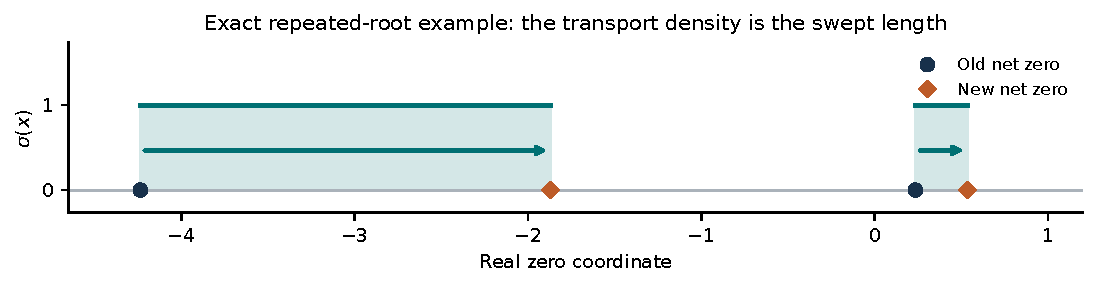
\includegraphics[width=\linewidth]{figures/finite_transport.pdf}
\caption{Exact finite example after common zero factors are cancelled
with their multiplicities.  The shaded area is total displacement.
The endpoints shown are the exact radicals given in the text.}
\end{figure}

For both polynomial examples, the script compares the exact determinant
phase with the sum of arctangent integrals over the moving intervals
and with numerical quadrature.  The largest recorded numerical
discrepancy was below $3\times10^{-66}$ at 180-digit working precision.
Exact symbolic identities and floating-point comparisons are separately
labelled in \texttt{data/verification.json}.

\subsection{Dirichlet and electrical transform checks}

For the ordinary construction, use the path Laplacian
\[
 A=\begin{pmatrix}1&-1&0\\-1&2&-1\\0&-1&1\end{pmatrix},
 \qquad B=(e_1-e_3)(e_1-e_3)^{\mathsf T},
\]
and inputs of conductors $1,3,4$, respectively.  The conductor-one input
is zeta; the other two are the real primitive characters.  Their
logarithmic derivatives at $iy$ are evaluated on the positive real
half-plane using the functional equation, the digamma function, and
finite Dirichlet sums.  The elementary tail bounds, for $s>1$, are
\[
 \left|\sum_{n>N}\frac{\chi(n)}{n^s}\right|
 \le\frac{N^{1-s}}{s-1},\quad
 \left|\sum_{n>N}\frac{\chi(n)\log n}{n^s}\right|
 \le N^{1-s}\left(\frac{\log N}{s-1}+\frac1{(s-1)^2}\right).
\]
The script records these truncation estimates and compares three-term
and 96-term matrix expansions.  The latter is used only in a region
where the matrix logarithm power series converges.

The ordinary normalized column below is
\[
 R_{\rm ord}(y)=\frac{\log y}{2\operatorname{tr}B}
                \operatorname{Im}\mathcal L_{A,B}(iy),
\]
whose limit is one.  For the squared construction, use three zeta inputs
on the same path and triangle, put $R=y^2$, and write $r(-R)$ for the
spanning-tree-normalized ratio in \eqref{eq:squared-stieltjes}.
The second normalization is
$R_{\rm sq}(y)=12\sqrt R\log r(-R)/\log R$, also with limit one.

\begin{center}
\begin{tabular}{rrr}
\toprule
$\log y$ & $R_{\rm ord}(y)$ & $R_{\rm sq}(y)$\\
\midrule
5   &0.64919196&0.63942986\\
10  &0.93622765&0.81627860\\
20  &1.01318185&0.90810615\\
50  &1.01626695&0.96324246\\
100 &1.00983903&0.98162123\\
200 &1.00532818&0.99081061\\
\bottomrule
\end{tabular}
\end{center}

\begin{figure}[ht]
\centering
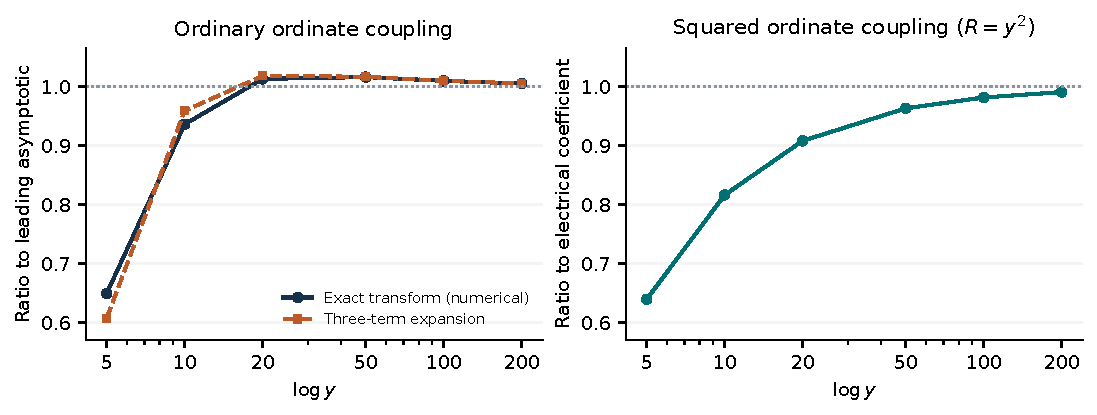
\includegraphics[width=\linewidth]{figures/transform_convergence.pdf}
\caption{Floating-point diagnostics of the exact transform formulas.
Each ratio tends to one.  These plots evaluate finite determinants and
positive-real Dirichlet expressions; they do not sum or certify an
infinite set of numerical zeros.}
\end{figure}

\subsection{What has and has not been checked}

The proofs of the transport constants, Poisson limit, moving-band local
law, and electrical companion were independently re-derived within this
research session.  The separate audit notes record the branch choice,
tail control, multiple-zero treatment, and squared-variable restriction.
They are mathematical review notes, not external peer review or formal
proof certificates.

The Python assertions passed.  Rational identities and root-isolation
checks are exact; mpmath output is not rigorously rounded.  Analytic
truncation bounds are supplied, but their decimal evaluations are not
interval certificates.  The unsmoothed and arbitrarily shrinking-band
claims rest on their proofs, not on the numerical figures.  No fresh
Lean build of the upstream theorem and no Lean formalization of the new
results is claimed.

The conductors, number of inputs, and graph matrices are fixed in the
matrix theorems.  The scalar theorem explicitly allows its tested value
interval to vary with $T$.  The squared theorem requires even inputs;
a single complex-character completion generally is not even.  No
consequence about all automorphic $L$-functions, new Euler products,
simple zeta zeros, or individual zero spacings is asserted.

\subsection{Reproducing the packet}

From the archive's top directory, run
\begin{verbatim}
python3 code/verify_transport.py
python3 code/make_figures.py
latexmk -pdf -interaction=nonstopmode paper.tex
\end{verbatim}
The first command regenerates the recorded JSON.  The second regenerates
the vector figures and PNG previews.  The third compiles this report
with a standard TeX Live installation.  A portable Python build helper
is also included for installations that have TeX sources but no generated
format or font map.  All source sections and figure assets needed to
compile the supplied document are in the archive.

For later formalization, the useful separation is: real canonical
products and strict half-plane sign; finite Hermitian inertia and matrix
logarithms; the positive Poisson rescaling lemma; and the Dirichlet
radial asymptotic.  The moving-window theorem then requires only scalar
integration and that rescaling lemma, while the electrical companion
adds the two-root forest identity and a positive Stieltjes Tauberian step.
This is a dependency plan, not a claimed executable Lean proof.
